\documentclass[a4paper]{usiinfbachelorproject}

\captionsetup{labelfont={bf}}
\usepackage{float}
\usepackage{amsmath}
\usepackage{graphicx}
\usepackage{enumitem}
\usepackage{booktabs}
\usepackage{hyperref}
\usepackage{listings}
\usepackage{tabularx}
\usepackage{placeins}
\usepackage{adjustbox}


\author{Polad Bakhishzade}

\title{\textbf{How Documentation Depth Influences LLMs' Ability to Judge Code Correctness}}
% \subtitle{Unveiling the Causes of Large-Language-Model Failures when Assessing Java Code}
\versiondate{\today}

\begin{committee}
  \advisor[Università della Svizzera italiana, Switzerland]{ }{Gabriele}{Bavota}
  \coadvisor[Università della Svizzera italiana, Switzerland]{ }{Giuseppe}{Crupi}
\end{committee}

% ——————————————————————————— ABSTRACT
\abstract{
Large Language Models (LLMs) are playing an increasingly significant role in software engineering tasks such as code generation, explanation, and bug fixing. A rapidly evolving application of LLMs is in the domain of automated code understanding—particularly in evaluating the functional correctness of code implementations. This task presents a challenging benchmark, as it requires the model to reason about both the code and its intended specification.\par\vspace{5pt} \noindent
This study explores how the quality and depth of natural-language documentation influence LLMs' ability to assess whether a Java function is correct. Specifically, we ask: \emph{To what extent does the richness and structure of natural language context affect an LLM's judgment of code correctness?}\par\vspace{5pt} \noindent
We extend the Java subset of the \textsc{CoderEval} code generation benchmark by systematically enriching the documentation of each problem with five structured documentation layers—ranging from brief summaries to formal pre/post-conditions. Our novel code understanding benchmark features 181 code generation problems. Each problem also features a correct and an incorrect candidate implementation (which are used to evaluate the models' abilities as a judge for code correctness), as well as five blocks of natural language documentation, each corresponding to a different level of detail. The documentation layers are designed to progressively enrich the context provided to the model, from a simple one-line summary (L1) to a full specification including behavioral descriptions, parameter explanations, examples, and formal constraints (L5). We then prompt three open-source LLMs—Qwen2.5-Coder-0.5B-Instruct, Qwen2.5-Coder-1.5B-Instruct, and DeepSeek-Coder-1.3B-Instruct—to act as zero-shot judges, under multiple prompt configurations, and evaluate their performances as code evaluators.\par\vspace{5pt} \noindent
Our results show that, despite the fact that all models struggle as judges of code correctness in zero-shot settings, the impact of added documentation varies significantly across models. Smaller models tend to benefit from concise descriptions but often struggle when faced with verbose or formalized inputs, leading to degraded performance. In contrast, larger models make better use of detailed specifications and exhibit improved judgment accuracy. Notably, some documentation layers—such as illustrative examples—can either aid understanding or introduce confusion, depending on the model.\par\vspace{5pt} \noindent
These findings underscore the need for model-aware prompt design when using LLMs for code understanding tasks. Importantly, the study challenges the assumption that more documentation always leads to better outcomes. Instead, it demonstrates that the type and presentation of natural language context must be carefully aligned with the model's input capabilities. These insights can guide the development of more effective LLM-based tools for software quality assurance.\\
\\[2pt]
\textbf{Keywords}: Software Engineering; Large Language Models; Prompt Engineering; Code Understanding Benchmark
}

\begin{document}
\maketitle
\tableofcontents\newpage

% ——————————————————————————— 1 INTRODUCTION
\section{Introduction}\label{sec:intro}
Large Language Models (LLMs) such as ChatGPT~\cite{openai2023chatgpt}, GitHub Copilot~\cite{githubcopilot}, and StarCoder~\cite{li2023starcoder} have become widely adopted in software development workflows. Originally developed for general language understanding, these models have rapidly gained traction in code-related tasks, including code generation, explanation, repair, and synthesis~\cite{jiang2024survey, chen2021codex, wang2023codet}. Researchers are increasingly exploring the use of LLMs for tasks such as debugging, static analysis, and functional correctness evaluation.\\
\\[2pt]
Among the many challenges in this space, one particularly important question is whether LLMs can serve as reliable evaluators of automatically generated code. In industrial settings, such as at Google, the proportion of code written or assisted by machine learning systems is steadily increasing. However, verifying the correctness of such code remains an open problem. Traditional techniques like writing unit tests are time-consuming and require substantial human effort, creating a bottleneck in workflows that rely heavily on automated code generation. Existing automatic evaluation metrics—such as BLEU~\cite{papineni2002bleu}, ROUGE~\cite{lin2004rouge}, METEOR~\cite{banerjee2005meteor}, and BERTScore~\cite{zhang2019bertscore}—have shown significant limitations in this setting. These metrics often rely on reference implementations, which may not be available, and struggle to capture functional equivalence between semantically correct but syntactically different solutions. Recent studies also highlight flaws in applying embedding-based metrics to code-related tasks~\cite{naik2024limitations}. This motivates the need for oracle-free evaluation mechanisms capable of assessing whether a candidate implementation adheres to a given specification.\\
\\[2pt]
While LLMs have shown strong performance in code generation, an open question remains: can they also reason about the correctness of code? This question has received relatively little attention so far, as most benchmarks are designed for code generation. Moreover, adapting code generation benchmarks for correctness evaluation is not trivial. Many such benchmarks provide only minimal or vague natural language descriptions, which are insufficient to test whether a model understands the functionality of the implementation it is evaluating.\\
\\[2pt]
In this work, we investigate how the judging abilities of LLMs vary with the depth and completeness of the instructions provided. Specifically, we create a correctness evaluation benchmark by extending the \textsc{CoderEval} dataset with five levels of natural language documentation. These range from a simple one-line summary of the function's purpose (L1), to a high-level description of the expected behavior and edge cases (L2), an explanation of the function signature and its parameters (L3), concrete input/output examples (L4), and formal pre- and postconditions specifying what must hold before and after execution (L5). We evaluate three instruction-tuned models—Qwen-0.5B, Qwen-1.5B, and DeepSeek-1.3B—across 362 function–candidate pairs. Each pair is tested under two conditions: \emph{cumulative prompts}, where the model sees all levels from L1 up to a given level, and \emph{ablation prompts}, where a specific level (e.g., L4) is removed from the full prompt to isolate its impact.\\
\\[2pt]
Our results suggest that the ability of LLMs to utilize different types of documentation varies across models. For instance, Qwen-1.5B shows a modest improvement in accuracy from 50\% to 55\% when provided with more detailed prompts, indicating some benefit from richer context. In contrast, smaller models like Qwen-0.5B and DeepSeek-1.3B exhibit inconsistent performance, sometimes declining with additional information. These findings suggest that prompt design can influence model performance, but its effectiveness varies: while richer prompts help some models slightly, others show inconsistent or even worse results.

\subsection*{Report structure}

Section~\ref{sec:related} reviews related literature.  
Section~\ref{sec:design} presents our study design and dataset enrichment pipeline.  
Section~\ref{sec:results} covers results from cumulative and ablation experiments.  
Section~\ref{sec:concl} concludes and outlines future directions.

% ——————————————————————————— 2 RELATED WORK
\section{Related Work}\label{sec:related}
As Large Language Models (LLMs) gain traction in software development, a growing body of research is investigating their potential not only as code generators but also as autonomous evaluators. Yet, assessing whether a model can reliably judge the correctness of code remains an open and challenging question. This section presents an overview of related efforts, focusing on the current limitations of LLM-based evaluation and recent benchmark development.\\
\\[2pt]
A key concern raised by recent work is that LLMs often lack deep semantic understanding of their own outputs. West et al.~\cite{west2023generative} formulate this as the “Generative AI Paradox”: models that generate impressive solutions may still fail to understand them. Their findings show that even top-tier LLMs frequently make overconfident yet incorrect predictions, especially on reasoning-intensive tasks. Gu et al.~\cite{gu2024counterfeit} expand this concern in the coding domain. They construct “counterfeit” solutions—plausible-looking but incorrect code—and show that LLMs often fail to flag these as erroneous. Instead, models are easily misled by surface-level cues and rarely recover from their own failures. Collectively, these studies highlight a core insight: evaluating code correctness is fundamentally distinct from generating code. Therefore, it is not safe to assume that a model which produces plausible-looking solutions is also a reliable evaluator of such completions.\\
\\[2pt]
Several studies have designed benchmarks to assess LLMs’ judgment ability in isolation. Zhao et al.~\cite{zhao2024codejudgeeval} introduce \textsc{CodeJudge-Eval}, a benchmark where LLMs must decide whether a given candidate solution is correct. The dataset includes subtle bugs, edge cases, and misleading code snippets. Across 12 models, including GPT-4 and Claude, accuracy remained low—rarely exceeding 60\%, with GPT-4 reaching at most 65\%. These results suggest that current models struggle with code correctness as a task, regardless of their size. Zhao et al. highlight that even advanced models like GPT-4 frequently misclassify incorrect solutions that contain subtle bugs or misleading logic. They suggest that reformulating the task—by giving more precise and complete descriptions of the expected behavior—and training models using datasets that include both correct and incorrect implementations could help improve judgment accuracy.\\
\\[2pt]
An influential approach is introduced by ICE-Score from Zhuo~\cite{zhuo2023icescore}, which suggests using GPT-3.5-turbo to evaluate candidate implementations using precisely crafted prompts that focus on properties such as correctness and readability. The study shows that prompting the model to explain its reasoning before delivering a final judgment enhances alignment with human evaluations.\\
\\[2pt]
Expanding on this idea, Tong and Zhang~\cite{tong2024codejudge} develop \textsc{CodeJudge}, a framework that builds on ICE-Score’s principles through a structured, multi-step evaluation process. In this setup, two instruction-tuned models are guided through reasoning stages—including explanation and justification—before returning a binary decision on correctness. Experiments reveal significant improvements in judgment accuracy across five datasets and programming languages, particularly for smaller models like Llama-3-8B-Instruct. In our study, we build on these insights but take a different angle: instead of structuring the reasoning steps, we structure the task description itself. By layering increasingly rich information—ranging from summaries to behavioral specifications and input/output examples—we investigate whether more detailed descriptions help models act as better judges.\\
\\[2pt]
While the studies above focus on correctness, others explore how to align model judgments with human coding preferences. Weyssow et al.~\cite{weyssow2024codeultrafeedback} introduce \textsc{CodeUltraFeedback}, a dataset of 10,000 coding problems, each answered by 14 different LLMs. These outputs are then ranked by GPT-3.5 across five dimensions: style, readability, instruction-following, complexity, and explanation. The authors use these rankings as training data to fine-tune CodeLlama-7B-Instruct, teaching it to prefer responses that GPT-3.5 rated more highly. The fine-tuned model is evaluated on HumanEval+~\cite{lzi2023humanevalplus}, where it outperforms the original base model in both preference alignment and functional accuracy. Although the task focuses on stylistic and qualitative assessment rather than functional correctness, the results suggest that training with ranked outputs can guide LLMs to better evaluate and generate code along desired dimensions such as style and readability.\\
\\[2pt]
A complementary line of research examines LLMs in educational settings. Koutcheme et al.~\cite{koutcheme2025evaluating} assess whether LLMs can generate and evaluate feedback on student code submissions in introductory Python assignments. Their goal is to explore how models can assist in automated grading systems that support student learning. They find that open-source models like StarCoder2 perform competitively with proprietary models such as GPT-4, particularly when provided with annotated student submissions that include instructor-written feedback, which serve as exemplars for what good feedback should contain. While not directly focused on correctness classification, this work supports the broader feasibility of using LLMs as evaluators of code quality.\\
\\[2pt]
In summary, the field is converging on the idea that LLMs can act as judges, but only under carefully crafted conditions. While prior work has focused on benchmarks, multi-step reasoning, or feedback alignment, our study lies in incrementally enriching the prompt descriptions and examining how models with different sizes respond to varying levels of contextual detail when judging code correctness.

% ——————————————————————————— 3 STUDY DESIGN
\section{Study Design}\label{sec:design}

\subsection*{Research Question}
\noindent\textbf{RQ –} \emph{To what extent does the quality and depth of natural language documentation affect the ability of LLMs to judge the correctness of a given Java function?}

\subsection{Context: LLMs}\label{sec:llms}
We selected three instruction-tuned large language models (LLMs) of relatively small size: \textbf{Qwen2.5-Coder-0.5B-Instruct}, \textbf{Qwen2.5-Coder-1.5B-Instruct}~\cite{qwen2024report}, and \textbf{DeepSeek-Coder-1.3B-Instruct}~\cite{deepseek2024report}. These models feature approximately 0.5, 1.5, and 1.3 billion trainable parameters respectively, which is three orders of magnitude smaller than the latest foundation models such as GPT-4, estimated to exceed one trillion parameters. We chose these smaller models to balance performance and computational feasibility, allowing us to run multiple evaluations on local academic hardware without relying on large-scale infrastructure. Although computational cost was not a formal constraint of the study, using smaller models made experimentation more feasible and reproducible in standard academic settings.\\
\\[2pt]
All three models are optimized for code-related tasks and released with instruction-following tuning, meaning they have been fine-tuned to generate appropriate responses to structured natural language instructions. This makes them well-suited for prompt-based evaluation tasks like the one in this study.\\
\\[2pt]
The term \emph{“Instruct”} indicates that the model has undergone additional fine-tuning on datasets that include natural language prompts and desired completions, making it more responsive to task-specific queries. The Qwen models are part of Alibaba’s Qwen2.5 series, designed for code tasks and instruction-following scenarios. Qwen2.5-Coder models were trained on a large mixture of public and synthetic datasets, including a multilingual corpus of code, technical Q\&A, and structured programming tutorials~\cite{qwen2024report}. In particular, Qwen2.5-Coder-1.5B was optimized for multi-task code understanding and generation, and supports fine-grained control over function-level behavior through instruction tuning.\\
\\[2pt]
DeepSeek-Coder is a family of decoder-only transformer models specifically built for programming-related tasks~\cite{deepseek2024report}. The DeepSeek-Coder-1.3B variant used in our study was pre-trained on a massive 2 trillion token corpus that includes 87.5\% code and 12.5\% natural language. It was then instruction-tuned on 2 billion tokens of high-quality problem–solution pairs and user queries. The model supports over 80 programming languages and is explicitly optimized for tasks such as code completion, explanation, and functional verification, making it suitable for prompt-based correctness evaluation.\\
\\[2pt]
All models were accessed via the Hugging Face Hub\footnote{\url{https://huggingface.co}}, an open-source platform that hosts pre-trained machine learning models and provides tools for deployment and evaluation. We used the Transformers library to run the models, which handled prompt tokenization, model loading, and inference (i.e., generating predictions) through a standardized API.

\subsection{Context: Dataset}\label{sec:dataset}
We based our experiments on the Java subset of the \textsc{CoderEval} benchmark~\cite{coderEval2023}, a code generation dataset containing 230 manually curated Java programming tasks. Each task includes: (i) a natural language specification describing what the function is expected to do, (ii) a reference implementation showcasing a possible correct solution, and (iii) an associated test suite for automated correctness verification. The output of each test suite is a boolean: \texttt{pass} indicates that a candidate satisfies all test cases, while \texttt{fail} indicates that it fails at least one.\\
\\[2pt]
Before adopting all 230 tasks, we performed a thorough quality assurance procedure to ensure the reliability of the test suites. This step was crucial, as test misbehavior could bias our evaluation—for instance, by incorrectly labeling an actually wrong solution as correct. We discarded 49 problems during quality control. Specifically, 20 tasks had reference implementations that failed their own test suites, indicating internal inconsistencies. Another 9 tasks had such weak test coverage that even empty functions passed all test cases. Additionally, 17 tasks were accepted by trivial dummy implementations, such as \texttt{return null;} or \texttt{return 0;}, which revealed a lack of discriminative power in the test suites. Finally, 3 tasks yielded inconsistent results for identical implementations across different evaluation runs. After filtering out these cases, we retained a final set of 181 Java tasks that passed all quality criteria and provided reliable correctness labels inferred directly from test outcomes.

\subsection{Data Collection}\label{sec:collection}

Although each problem in the dataset includes a natural language docstring, these descriptions are often minimal—typically consisting of a single vague sentence. For example: “Performs a right node rotation.” or “Skips bytes until the end of the current line.”\\
\\[2pt]
Since our goal is to evaluate the extent to which the quality and depth of natural language documentation affect the ability of LLMs to judge the correctness of a given Java function, the one-line documentation featured in the \textsc{CoderEval} dataset is insufficient to answer this question. For this reason, we augmented the description of each code generation problem with a five-layer natural language description covering different aspects of code documentation, such as parameter explanations and examples of input–expected output pairs.

\subsubsection{Augmenting the Dataset}\label{sec:augmentation}
Our goal is to study the extent to which the natural language documentation affect the ability of LLMs to judge the correctness of Java functions. To enable this evaluation, we enriched the \textsc{CoderEval} dataset with additional structured documentation, since the original format was designed for code generation, not understanding.\\
\\[2pt]
We used GPT-4o to produce this documentation because it was both scalable and accurate. Manual annotation of all 181 Java functions across multiple levels would have been impractical, and GPT-4o consistently followed structured formatting and stylistic constraints when prompted correctly.\\
\\[2pt]
Each prompt to GPT-4o included the full Java function body and its name. The model was asked to return a five-part structured description covering different semantic aspects of the function:

\begin{enumerate}[leftmargin=15pt]
  \item[\textbf{L1}] \textbf{Summary}: a concise one-sentence description of the function's high-level purpose, strictly excluding edge cases.
  \item[\textbf{L2}] \textbf{Behavioral description}: a 1--2 sentence narrative detailing the function’s logic, including how edge cases and special conditions are handled.
  \item[\textbf{L3}] \textbf{Signature explanation}: structured tags describing the meaning of each parameter and the return value (\texttt{@param}, \texttt{@return}, \texttt{@throws}), if applicable.
  \item[\textbf{L4}] \textbf{Examples}: several one-line input–output pairs with explanatory notes clarifying expected behavior.
  \item[\textbf{L5}] \textbf{Preconditions and postconditions}: short logical statements capturing required input constraints and expected output guarantees.
\end{enumerate}
The outputs followed a fixed format and were manually verified for quality and correctness. We ensured that L1 remained high-level, L2 captured the full logic and edge cases, and L3–L5 remained accurate, relevant, and specific to each function. This enrichment gave us modular “building blocks” that could be flexibly combined into prompts with different levels of information. For example, combining L1 and L2 produces a compact explanation of the function’s purpose and behavior, while L1 and L3 give purpose plus interface-level understanding without relying on examples or full logic. This modularity was essential for constructing the incremental and layer-removal settings used in our evaluation.\\
\\[2pt]
To make this enrichment structure more concrete, we present a full example based on one of the tasks from the dataset. We selected this method because its original documentation is completely uninformative, consisting only of a JavaDoc inheritance marker without any description of behavior or output. This makes it especially suitable for demonstrating how enrichment reveals semantics hidden from both humans and LLMs.

\clearpage
\begin{lstlisting}[language=Java, caption={Reference implementation of \texttt{previousNode}}, label={lst:previous}]
@Override 
public ListNode<E> previousNode(){
  checkForComodification();
  if (!hasPrevious()) {
    throw new NoSuchElementException();
  }
  last = next = next.prev;
  nextIndex--;
  return last;
}
\end{lstlisting}
The original \textsc{CoderEval} docstring was entirely absent, containing only an inheritance placeholder without any task-specific detail:

\begin{flushleft}
\ttfamily
\small
/\** \\
\{@inheritDoc\}\\
*\ /
\end{flushleft}
To compensate for this lack of context, we prompted GPT-4o to generate five structured enrichment layers that clarify the method’s logic, behavior, and usage. Each layer adds detail to the prompt, helping the model reason about preconditions, logic, and edge cases:\\
\\[2pt]
\textbf{L1 – Summary:} Returns the previous node in a doubly linked list.\\[2pt]
\textbf{L2 – Behavioral description:} Checks for concurrent modifications, verifies availability of a previous node, then updates and returns the previous node.\\[2pt]
\textbf{L3 – Signature explanation:}
\begin{quote}\ttfamily
@return ListNode<E>: The previous node in the list.\\
@throws NoSuchElementException: If no previous node exists.
\end{quote}
\textbf{L4 – Examples:}

\begin{center}
\renewcommand{\arraystretch}{1.2}
\begin{tabular}{@{}l@{\hskip 1em}l@{}}
current node \textrightarrow\ previous node & (navigates backwards) \\
start of list \textrightarrow\ exception & (throws if no previous node)
\end{tabular}
\end{center}
\textbf{L5 – Preconditions and postconditions:} List must not be concurrently modified, cursor must not be at the list start; post-execution, cursor steps back one node.

\subsubsection{Building Candidate Pairs}\label{sec:judgments}
For each of the 181 Java problems, we generated multiple candidate implementations using several large language models, including DeepSeek-Coder-6.7B~\cite{deepseek2024report} and Qwen2.5-Coder-7B~\cite{qwen2024report}. These completions were collected into a custom knowledge base containing over 5,000 generated solutions.\footnote{\url{https://github.com/poladbachs/Bachelor-Thesis/blob/main/CoderEval/knowlbase_codereval.csv}} We then ran the test suites of \textsc{CoderEval} on these candidates and assigned to each of them a ground truth label: 1 if the implementation was correct, or 0 if it was incorrect.
\\[2pt]
We applied a filtering process to remove trivial, duplicate, or unusable code. First, we discarded placeholder code such as \texttt{/* implementation goes here */} or empty function bodies, which clearly lacked any executable logic. Second, we excluded logic-less shells like \texttt{return;} or \texttt{return 0;} that performed no computation and could not plausibly be evaluated for correctness. Third, we removed print-only stubs such as \texttt{System.out.println("TODO");}, as these were clearly placeholders and not real attempts at implementation. Fourth, we eliminated duplicate implementations to ensure that each candidate pair provided a distinct comparison case. Finally, we removed candidates that relied on methods, classes, or functionality not defined within the task scope. For example, some generated implementations contained comments such as:
\begin{quote}\ttfamily\small
// Assuming there's a getDefaultValue method for the class\\
// Assuming IsomorphicGraphMapping is a custom class\\
// Update heights (assuming that updateHeight() is defined)
\end{quote}
Such phrases indicate that the code presumes the existence of external dependencies that are not guaranteed to be available within the function's context. Including these candidates would introduce ambiguity, as correctness could no longer be determined purely based on the prompt and provided code. We therefore excluded all such cases to maintain a closed-world evaluation setup, where all necessary information is explicitly present.\\
\\[2pt]
After filtering, we finalized the dataset by selecting one correct and one incorrect implementation per problem. When no valid correct candidate was found, we fell back to using the original reference implementation from \textsc{CoderEval}. In two exceptional cases where no usable incorrect candidates were available, we manually inserted a faulty variant into the dataset to complete the correct–incorrect pairing.

\subsection{Prompting and Evaluation Setup}\label{sec:evaluation}
Each model was tasked with a binary classification problem: given a natural language description, a function signature, and a candidate implementation, it must decide whether the implementation correctly satisfies the described behavior. The model is asked to output \texttt{1} if the implementation is correct, and \texttt{0} otherwise.
The exact prompt given to the models was formatted as follows, using placeholders to insert task-specific information:

\begin{quote}\ttfamily
You will be provided with the description ("Description") and the signature ("Signature") of a Java function to implement. You will also see a candidate implementation ("Candidate"). Your role is to evaluate the correctness of the Candidate, providing as output either 0 or 1, and no other text:

0. Wrong Implementation: The implementation does not correctly implement the described function.\\
1. Correct Implementation: The implementation correctly implements the described function.

\# Description:\\
\{Description\}

\# Signature:\\
\{First line of target implementation\}

\# Candidate:\\
\{Full candidate implementation\}

\# Output:
\end{quote}
The \texttt{\{Description\}} placeholder may contain varying levels of structured documentation depending on the experiment (from a one-line summary (L1) to the pre/post conditions (L5)).\\
The \texttt{\{First line of target implementation\}} refers to the method signature and is always identical to the candidate’s, as we discarded all candidates with mismatched signatures.
All prompts were encoded and passed to the models using Hugging Face Transformers with temperature set to 0.2. This low temperature was chosen to reduce randomness, since we could not afford to run multiple evaluations on the same instance. A limit of \texttt{max\_new\_tokens = 20} was enforced to constrain output length and prevent verbose completions, as the task only required a single-digit response (0 or 1). Model outputs were parsed to extract a binary classification, and any non-conforming output was treated as invalid and recorded as \texttt{None}.\\
\\[2pt]
We evaluated model performance under two experimental settings. In both, the baseline was the minimal prompt containing only the L1 summary layer.\\
\\[2pt]
In the first setting, prompt enrichment, we incrementally increased the amount of documentation information provided to the model. Starting from L1 alone, we progressively added layers in the following order: L2 (behavioral explanation), L3 (signature-level tags), L4 (input–output examples), and finally L5 (logical constraints). This yielded five prompt configurations per model, corresponding to L1, L1+L2, L1+L2+L3, L1+L2+L3+L4, and the full L1–L5 stack. We applied this setup to three LLMs—Qwen-0.5B, Qwen-1.5B, and DeepSeek-1.3B—resulting in 15 experiments in total.\\
\\[2pt]
In the second setting, layer removal, we started from the full prompt containing all five documentation layers (L1–L5) and selectively removed individual or combined layers to assess their individual effect on model performance. Rather than exhaustively testing all combinations, we defined a limited set of configurations per model to observe the contribution of each layer. This experimental approach helped isolate which layers had the greatest impact on accuracy and whether some components could be omitted without harming performance. The detailed discussion of results is presented in Section~\ref{sec:results}.

\subsection{Data Analysis}\label{sec:analysis}

Each model was evaluated on a binary classification task: given a natural language description of a Java function and a candidate implementation, decide whether the implementation correctly satisfies the described behavior. Ground truth correctness labels were derived by running the \textsc{CoderEval} test suites on each candidate, as described in Section~\ref{sec:judgments}. \\
\\
Using these two independent sources—predefined correctness labels and model predictions—we computed standard confusion matrix metrics. A true positive (TP) occurs when the model correctly identifies a correct implementation. A true negative (TN) is when the model correctly identifies an incorrect implementation. A false positive (FP) occurs when the model labels as correct an implementation that fails the test suite. A false negative (FN) occurs when the model labels as incorrect an implementation that passes the test suite.\\
\\[2pt]
Because our dataset was balanced—containing 181 correct and 181 incorrect implementations—we report accuracy as the primary performance metric. Accuracy reflects the overall proportion of correct classifications (TP and TN) over all evaluated samples:
\[
\text{Accuracy} = \frac{TP + TN}{TP + TN + FP + FN}
\]
Model outputs that did not include a valid binary prediction (\texttt{0} or \texttt{1}) were marked as invalid and excluded from metric calculations.

% ——————————————————————————— 4 RESULTS
\section{Results \& Discussion}\label{sec:results}

\subsection{Incremental Enrichment (L1 $\rightarrow$ L5)}

To assess how progressively detailed documentation impacts model performance, we first examine the cumulative enrichment results shown in Figure~\ref{fig:acc-l1-l5}. Each model was evaluated across five prompt variants, from the minimal summary-only setting (L1) to the full specification (L1–L5), revealing distinct behavioral patterns across models.

\begin{table}[htbp]
\centering
\caption{Number and percentage of invalid model judgments (i.e., outputs not equal to 0 or 1) for each prompt variant. Each column represents a cumulative enrichment level: e.g., L1–L3 includes summary (L1), behavioral description (L2), and method signature (L3). Percentages are computed over the full set of 362 evaluated function pairs.}
\begin{tabular}{lccccc}
\toprule
\textbf{Model} & \textbf{L1} & \textbf{L1-L2} & \textbf{L1-L3} & \textbf{L1-L4} & \textbf{L1-L5} \\
\midrule
Qwen 2.5 Coder 0.5B & 2 (0.6\%) & 0 (0.0\%) & 0 (0.0\%) & 5 (1.4\%) & 2 (0.6\%) \\
Qwen 2.5 Coder 1.5B & 1 (0.3\%) & 0 (0.0\%) & 0 (0.0\%) & 0 (0.0\%) & 0 (0.0\%) \\
DeepSeek Coder 1.3B & 11 (3.0\%) & 15 (4.1\%) & 20 (5.5\%) & 51 (14.1\%) & 70 (19.3\%) \\
\bottomrule
\end{tabular}
\label{tab:invalid-judgments}
\end{table}

\noindent
Table~\ref{tab:invalid-judgments} shows that DeepSeek Coder 1.3B exhibits a sharp increase in invalid judgments as more layers are added, peaking at nearly 20\% at L5. In contrast, both Qwen models maintain a low invalid rate across settings, with Qwen 2.5 Coder 1.5B producing no invalid predictions beyond L1. 

\begin{figure}[H]
  \centering
  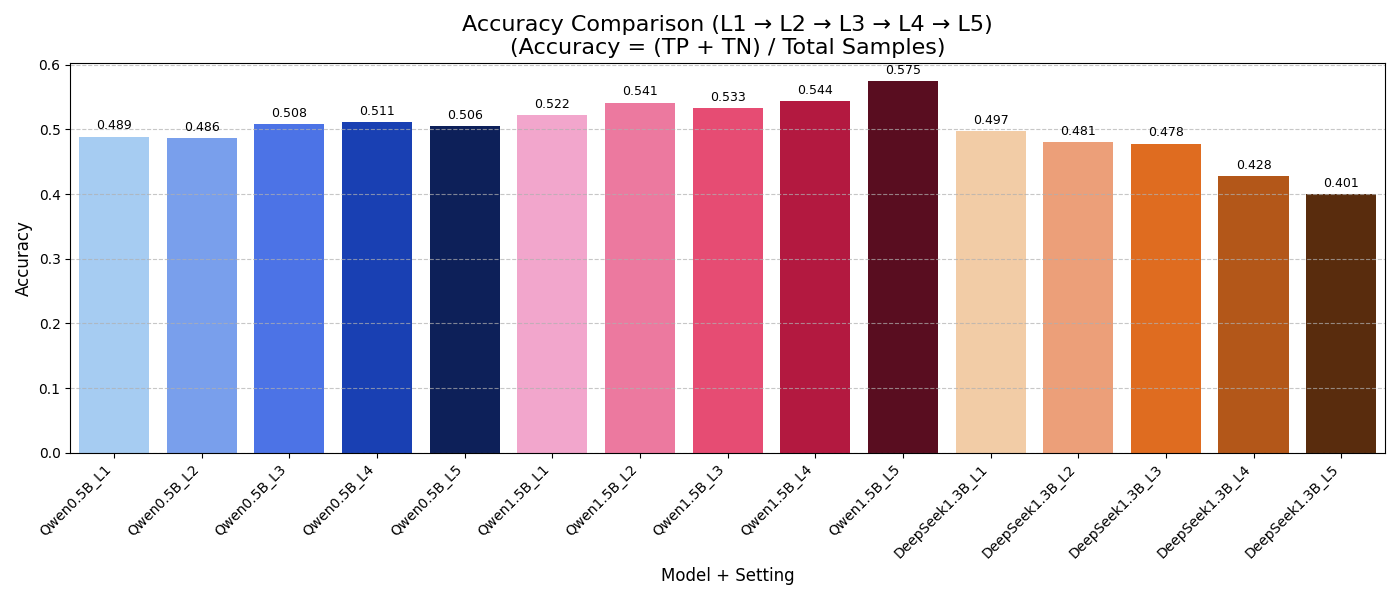
\includegraphics[width=\linewidth]{./figures/accuracy_comparison.png}
  \caption{Accuracy comparison across cumulative prompt settings. Each model is tested from L1 to L5.}
  \label{fig:acc-l1-l5}
\end{figure}
\noindent
The smallest model, Qwen-0.5B, starts at an accuracy of 0.49 with only the summary (L1) and fails to gain meaningful improvement through L2. However, accuracy rises once signature explanations (L3) and concrete examples (L4) are introduced, reaching a peak of 0.51. The final documentation layer (L5), which introduces formal logical conditions, causes a slight performance drop. This pattern suggests that Qwen-0.5B benefits from moderate enrichment, particularly when structural or procedural cues are provided, but may be overwhelmed by overly formal content. \\
\\
Qwen-1.5B, with three times the parameter count of 1.5 billion, exhibits a markedly different trajectory. It improves with each successive layer, rising from 0.52 at L1 to 0.57 at L5, a total improvement of 5.3\%. The gains are smooth and incremental but remain modest overall, indicating that while this model is capable of integrating richer, layered context, the improvement is limited in absolute terms. Notably, there is a slight dip at L3, where performance temporarily decreases before recovering with L4 and L5. This suggests that the inclusion of method signature descriptions may affect the model’s estimation of the most probable next token, leading to reduced accuracy. Unlike Qwen-0.5B, however, Qwen-1.5B shows no degradation with the introduction of preconditions or postconditions, suggesting a higher tolerance for semantic complexity. \\
\\
DeepSeek Coder 1.3B shows no consistent benefit from documentation enrichment. Accuracy starts at 0.51 under the minimal L1 prompt and fluctuates slightly with each additional layer, ending at 0.49 under the full L1–L5 prompt. The variation across all settings remains within a narrow 1.6 percentage point range, suggesting that the model is largely unaffected by prompt composition. Overall, the results indicate that documentation layering has little impact on DeepSeek’s ability to assess functional correctness in a zero-shot classification task.

\subsection{Model Behavior via Confusion Matrix Metrics}
To better understand these contrasting dynamics, we inspect the confusion matrix decomposition of model predictions across the enrichment levels. Figures~\ref{fig:qwen05-matrix},~\ref{fig:qwen15-matrix}, and~\ref{fig:deepseek-matrix} report true positives (TP), true negatives (TN), false positives (FP), and false negatives (FN) for Qwen-0.5B, Qwen-1.5B, and DeepSeek-1.3B respectively.
\begin{figure}[H]\centering
  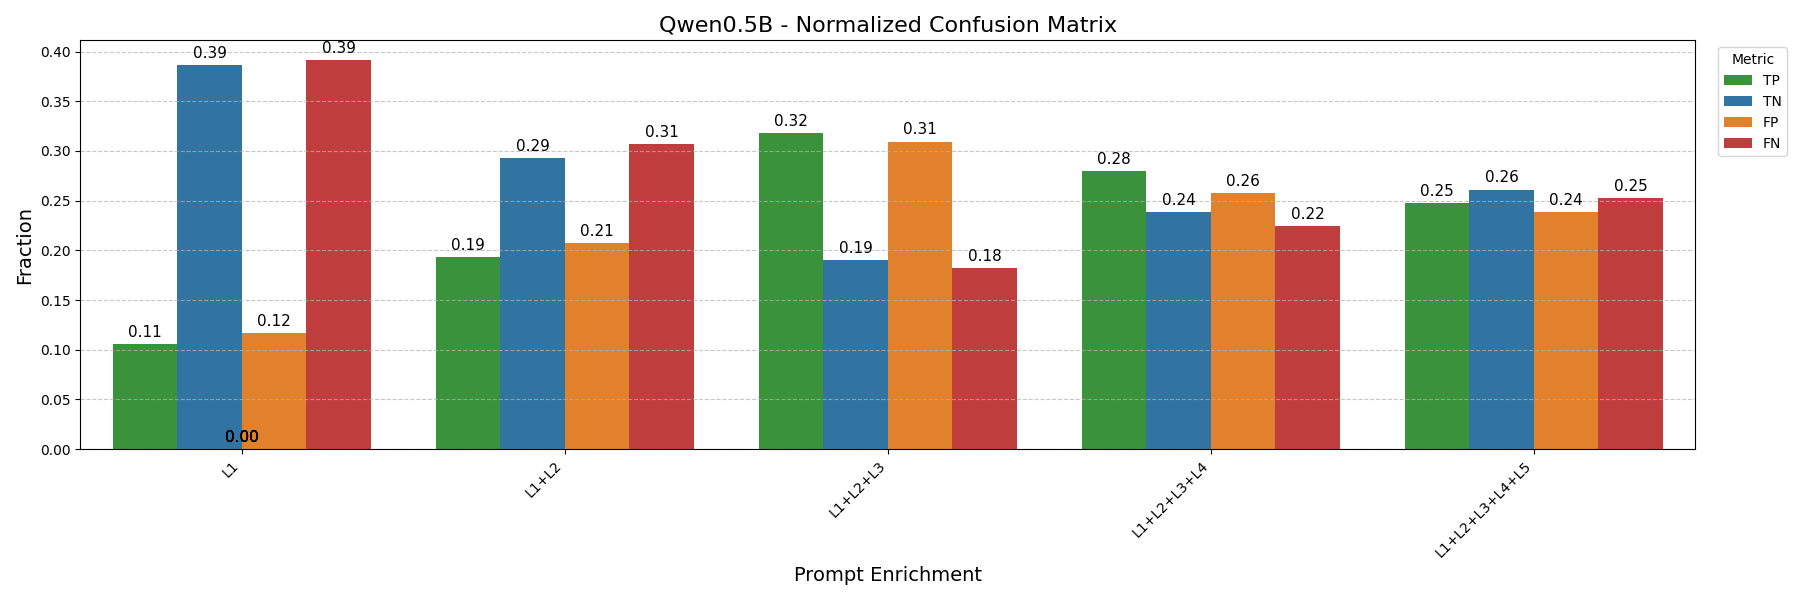
\includegraphics[width=\linewidth]{figures/Qwen0.5B_matrix.png}
  \caption{Normalized confusion-matrix metrics for Qwen-0.5B across L1 to L5.}
  \label{fig:qwen05-matrix}
\end{figure}
\noindent
Qwen-0.5B demonstrates a high number of false negatives under the L1 (summary-only) and L1+L2 (summary plus behavioral description) prompts. These values are expressed as fractions of the total set of judged implementations: for example, a false negative rate of 0.39 means that 39\% of all correct implementations were incorrectly classified as incorrect. At L1 and L1+L2, the false negative rates are 0.39 and 0.31, respectively. When signature information is introduced at L3 (i.e., L1+L2+L3), the false negative count drops to 0.18, and true positives increase to 0.32, indicating that lightweight structural context can support more effective predictions. However, further enrichment leads to a decline in performance. At L4 (with examples), true positives decrease (to 0.28) and false negatives rise again (to 0.22), while true negatives increase slightly to 0.24, possibly reflecting improved rejection of incorrect candidates. At the fully enriched L5 prompt (which includes logical preconditions and postconditions), the model becomes increasingly conservative: false negatives continue to rise (to 0.25) and true positives fall (to 0.25). Overall, while L3 offers some benefits, the addition of L4 and L5 does not improve performance and may reduce Qwen-0.5B’s ability to recognize correct implementations.
\begin{figure}[H]\centering
  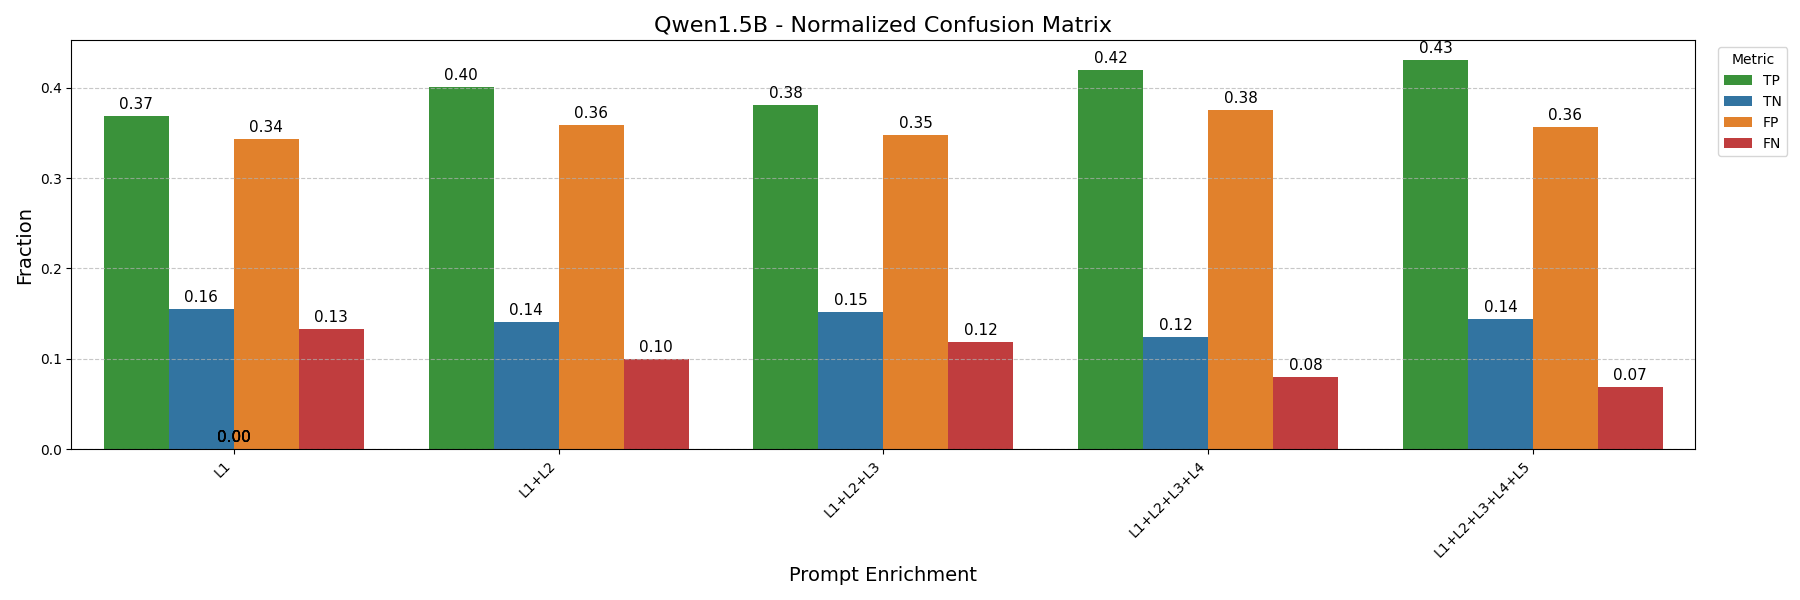
\includegraphics[width=\linewidth]{figures/Qwen1.5B_matrix.png}
  \caption{Normalized confusion-matrix metrics for Qwen-1.5B across L1 to L5.}
  \label{fig:qwen15-matrix}
\end{figure}
\noindent
Qwen-1.5B shows a mild improvement as more documentation is added, with true positives increasing from 0.37 at L1 (summary-only) to 0.43 at L1–L5 (full prompt), and false negatives dropping from 0.13 to 0.07. A slight dip occurs at L3: true positives decrease from 0.40 (at L1–L2) to 0.38, while true negatives and false negatives both slightly increase (TN to 0.15, FN to 0.12). This suggests that the inclusion of method signature descriptions may affect the model’s estimation of the most probable next token, leading to mildly reduced accuracy. After L3, true positives increase again (to 0.42 and 0.43), while false negatives continue to decline. After adding L4 and L5, false positives also rise slightly from 0.34 to 0.36. These shifts are small, but together they indicate that Qwen-1.5B integrates enrichment layers somewhat more effectively than Qwen-0.5B, maintaining stable or slightly improved recognition of correct implementations across prompt variants.
\begin{figure}[H]\centering
  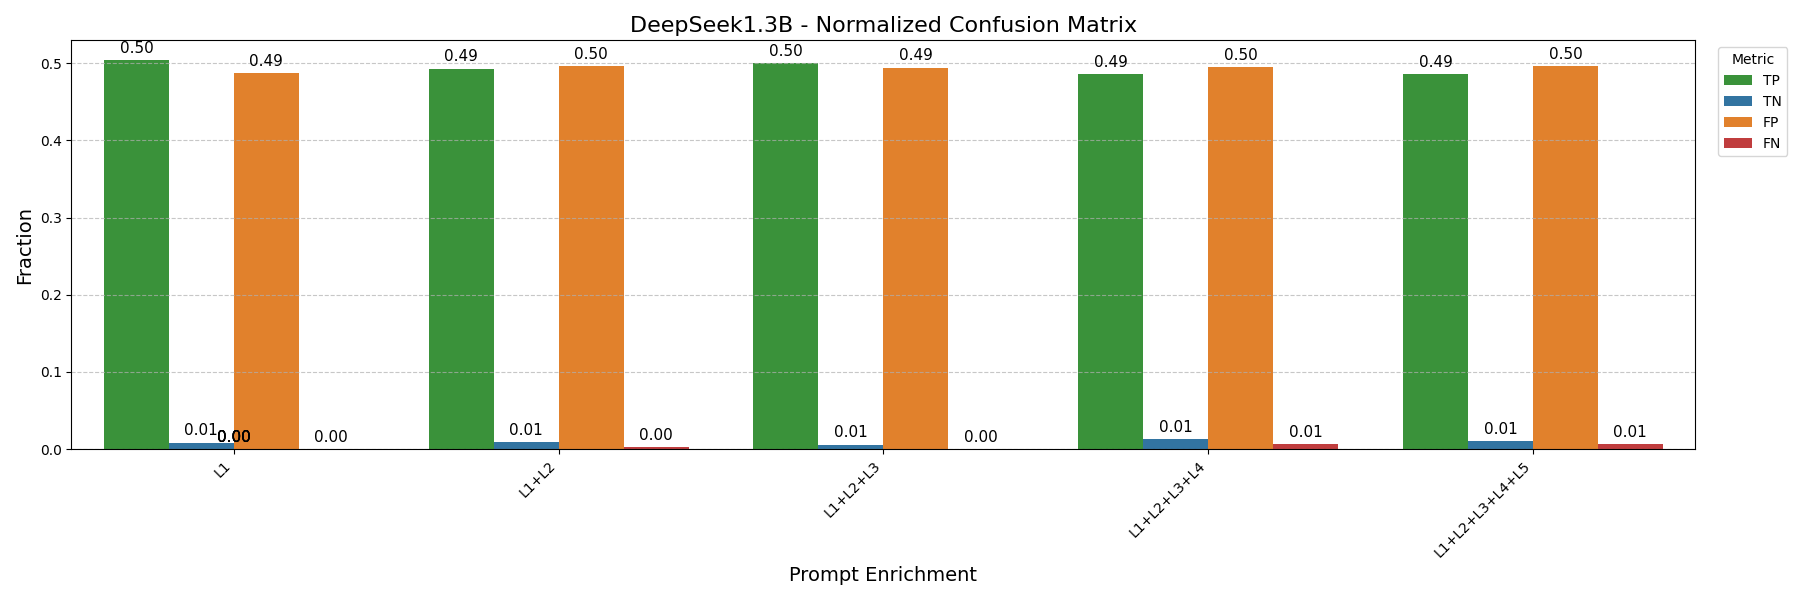
\includegraphics[width=\linewidth]{figures/DeepSeek1.3B_matrix.png}
  \caption{Normalized confusion-matrix metrics for DeepSeek-1.3B across L1 to L5.}
  \label{fig:deepseek-matrix}
\end{figure}
\noindent
DeepSeek Coder 1.3B behaves like a constant classifier. Across all enrichment levels, it predicts almost all implementations as correct, resulting in consistently high true positive (TP) and false positive (FP) rates—both fluctuating narrowly between 0.49 and 0.50—with near-zero true negatives (TN). The inclusion of additional documentation layers has no clear effect on these distributions. These results indicate that DeepSeek does not meaningfully adapt its behavior in response to richer prompts.

\subsection{Documentation Layer Removal}
The previous section highlighted how documentation enrichment impacts model behavior, with some layers providing slight benefit and others introducing instability. To better understand these effects, we now turn to targeted layer removals. The aim is to isolate the contribution of individual components and evaluate whether reduced prompts can maintain comparable performance to the fully enriched setting.\\
\\
Layer removal configurations were selected based on behavioral trends observed in Section~\ref{sec:results}. For Qwen 0.5B, we focused on removing L2, L4, and L5—layers that previously caused notable fluctuations in prediction quality. For Qwen 1.5B, L1 appeared consistently redundant, so all compound removals begin with its exclusion. For DeepSeek 1.3B, we excluded L2 and L4, which appeared to degrade reliability and increase invalid responses as shown in Table~\ref{tab:ablation-invalids}. We did not test arbitrary combinations such as removing L3 and L5, as no specific degradation patterns were observed when those layers were included, In fact, for Qwen 1.5B, the addition of L5 led to a 3\% increase in accuracy—a comparatively decent gain given the overall scale of variation, reinforcing its potential benefit rather than suggesting removal. \\
\\
Having assessed the impact of our documentation enrichment strategy on the performance of LLMs judging the code correctness, we now isolate the impact of individual layers through selective removal from the full prompt containing all five documentation layers (L1–L5). Figure~\ref{fig:ablation-accuracy} displays model accuracy under selective documentation removal, with one or more layers omitted from the full prompt.\\

\begin{table}[H]
\centering
\small
\begin{tabular}{lcc}
\toprule
\textbf{Model} & \textbf{Layer Removal Setting} & \textbf{Invalid Outputs (None)} \\
\midrule
Qwen 2.5 Coder 0.5B & - L1 & 0 (0.0\%) \\
                    & - L2 & 5 (1.4\%) \\
                    & - L1 - L4 & 0 (0.0\%) \\
                    & - L1 - L4 - L5 & 1 (0.3\%) \\
Qwen 2.5 Coder 1.5B & -L1, -L1-L4, -L1-L5, L1-L3 & 0 (0.0\%) \\
DeepSeek Coder 1.3B & - L2 & 56 (15.5\%) \\
              & - L2 - L4 & 23 (6.4\%) \\
              & - L2 - L4 - L5 & 25 (6.9\%) \\
\bottomrule
\end{tabular}
\caption{Invalid (None) outputs under selective layer removals. All percentages are computed out of 362 candidate evaluations per setting.}
\label{tab:ablation-invalids}
\end{table}
\noindent
Table~\ref{tab:ablation-invalids} shows invalid output rates under selected layer removals. Qwen 1.5B produces no invalid outputs in any setting. Qwen 0.5B is mostly stable, with minor issues under –L2 (1.4\%) and –L1–L4–L5 (0.3\%). DeepSeek 1.3B shows the most instability: removing just L2 causes 15.5\% invalids, while compound removals still result in 6–7\% failure rates.

\begin{figure}[H]\centering
  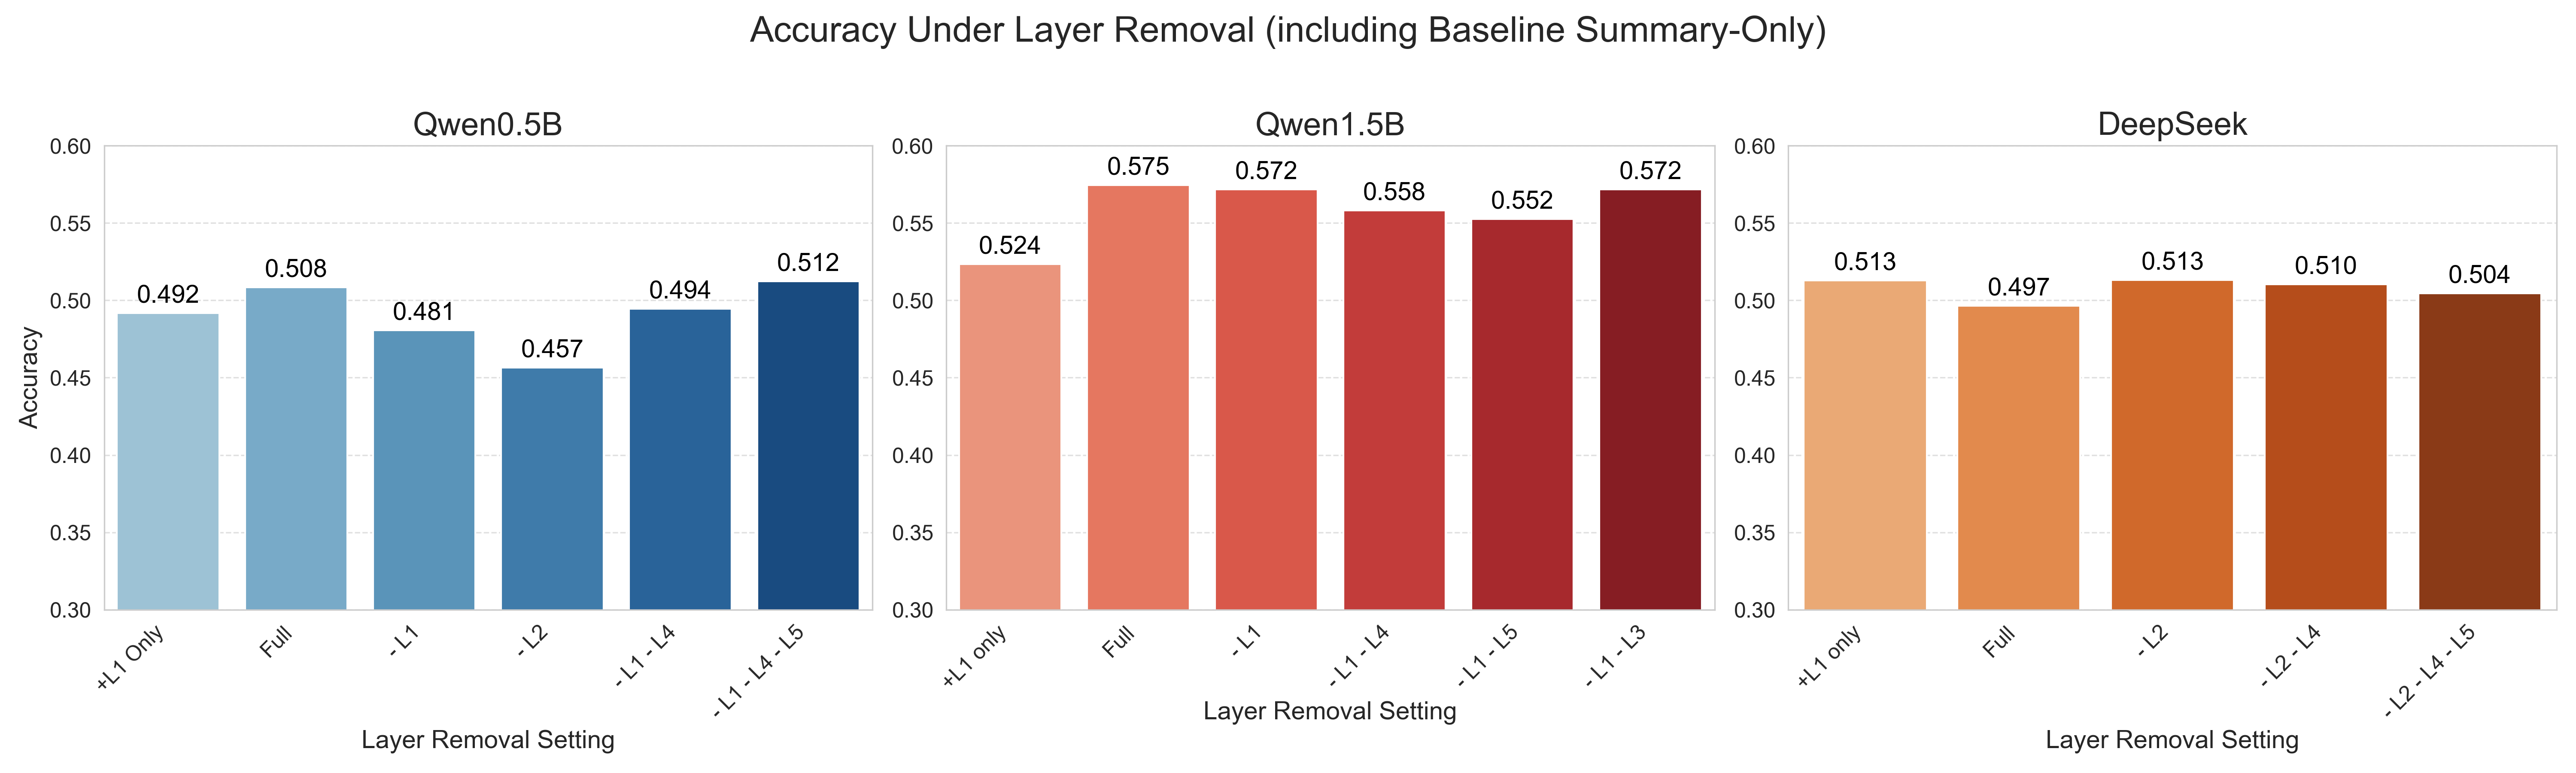
\includegraphics[width=\linewidth]{./figures/ablation_accuracy_subfigs.png}
  \caption{Accuracy after removing selected layers from the full prompt.}
  \label{fig:ablation-accuracy}
\end{figure}
\noindent
Removing the behavioral layer (L2) causes the most significant accuracy drop for Qwen 0.5B, reducing performance from 0.50 to 0.45. This confirms that functional behaviour can be relatively helpful to the model's success. Interestingly, removing the summary (L1) has a minor effect, suggesting that Qwen 0.5B does not depend heavily on introductory one-liner, since it already has a detailed description (L2). While removing only L1 or L1 and L4 yields 0.48 and 0.49 respectively, removing L1, L4, and L5—leaving only the behavioral and signature layers (L2 and L3)—achieves 0.51, slightly outperforming the full-prompt setting. This suggests that cutting certain prompt layers can help avoid the noise introduced by further layers. Note, however, that this improvement of 2\% is only marginal compared to the summary-only baseline at 0.49. \\
\\
Qwen 1.5B, in contrast, maintains a flat accuracy regardless of which individual layer is removed. The worst-case drop—removing L1 and L4—only reduces accuracy from 0.57 to 0.55. This demonstrates that no single layer is essential for the model to perform well and suggests that Qwen 1.5B can extract sufficient meaning from the remaining context when any one component is missing. Notably, removing L1 has almost no effect, confirming that this summary layer is redundant at this model size. For this reason, we exclude L1 in all compound removal scenarios and instead focus on testing the impact of removing richer content (L4, L5) under a reduced setting. The findings support the view that Qwen 1.5B integrates context holistically and can remain robust under prompt variation, even when trimmed. We also find that removing L3 alongside L1 yields no accuracy loss, reinforcing the minimal influence of the method signature layer in this model. \\
\\
DeepSeek 1.3B shows minimal sensitivity to individual layer removals. Accuracy remains roughly flat across all configurations, ranging from 0.49 (full prompt) to a modest peak of 0.513 under –L2. Compound removals such as –L2–L4 or –L2–L4–L5 result in small fluctuations but do not improve the model’s ability to distinguish correct from incorrect implementations.

\section{Conclusions \& Future Work} \label{sec:concl}
The three models tested in this study—Qwen 0.5B, Qwen 1.5B, and DeepSeek 1.3B—performed poorly across all prompt configurations, with no setting exceeding 58\% accuracy. These results indicate that, in a zero-shot setting, the tested models cannot be practically used for assessing the correctness of code, even when provided with structured natural language documentation.\\
\\
This study aimed to explore how different types of documentation influence the ability of language models to judge the functional correctness of Java code. To that end, we constructed an evaluation pipeline that progressively enriched function descriptions with five layered components—ranging from brief summaries to formal preconditions and postconditions. We then tested three instruction-tuned LLMs of varying size—Qwen 0.5B, Qwen 1.5B, and DeepSeek 1.3B—on both cumulative enrichment and selective removal variants of these prompts. \\
\\
Across 362 candidate pairs, we evaluated each model's binary judgments using accuracy and confusion matrix analysis. The results showed that prompt effectiveness is not uniform but deeply model-dependent. Qwen 0.5B benefited most from lightweight yet specific input: it achieved peak performance when provided only with the behavioral specification and the method signature (L2+L3), while further enrichment with examples and logical constraints introduced noise and reduced reliability. In contrast, Qwen 1.5B demonstrated robust improvements across the full prompt hierarchy, tolerating verbosity and integrating context holistically. DeepSeek 1.3B, on the other hand, consistently struggled regardless of prompt structure. Accuracy remained low across all configurations, and enrichment with additional documentation layers did not lead to improvements. In some cases, removing select components such as L2, L4, and L5 produced marginal gains, but the overall pattern indicates limited capacity to use either concise or verbose prompts effectively. \\
\\
In practical terms, these results show that optimal prompt design is not one-size-fits-all: each model responds differently to documentation structure. Smaller models such as Qwen-0.5B benefit from focused functional cues (L2+L3), while larger ones such as Qwen-1.5B tolerate verbosity. DeepSeek-1.3B, by contrast, appears largely unresponsive to prompt structure.

\subsection*{Future Work}
Several directions remain open for future exploration. First, our evaluation was static: models were asked to classify correctness using fixed input pairs, without follow-up clarification or iterative reasoning. Future work could investigate dynamic prompting strategies, such as presenting labeled examples before classification or incorporating intermediate feedback signals—e.g., using model confidence scores or tool-generated hints—to guide the model during the decision process. \\
\\
Second, our correctness labels were based strictly on the test suite's exit code. While this binary scheme captures functional correctness in most cases, it does not distinguish between fully correct and partially correct implementations—e.g., solutions that pass core functionality but fail rare edge cases. Future evaluations could explore more nuanced supervision signals. For example, semantic equivalence scoring—as explored in CodeXGLUE~\cite{Lu2021codexglue}—compares the behavior of two programs across a diverse set of inputs rather than relying on a fixed test suite. Alternatively, human-in-the-loop evaluation could involve expert annotators scoring implementations on correctness and clarity, providing richer feedback than pass/fail outputs alone~\cite{smith2021human}. \\
\\
Third, our analysis focused on three small to moderately sized open models due to resource constraints. Including larger models, such as GPT-4 or Claude (Anthropic's large language model~\cite{claude2023blog}), could clarify whether the trends we observed generalize to higher-capacity systems or are limited to the models tested here.\\
\\
Finally, additional research could examine failure patterns in more detail—for instance, when and why specific layers like L4 or L5 confuse a model. Understanding such breakdowns could help define safer and more effective prompt templates for future applications in code assessment or feedback generation.\\
\\
In conclusion, this study demonstrates that not all layers of natural language documentation contribute equally to model accuracy. Some forms of enrichment help even though still moderately, while others may dilute or obscure the underlying intent. Prompting strategies should therefore be designed with model-specific behaviors in mind, not based on the assumption that more detail always leads to better results.\\

\subsection*{Replication Package}\label{sec:replication}
All source code, enriched datasets, model evaluation scripts, and plotting tools are available in the following GitHub repository:
\begin{center}
\url{https://github.com/poladbachs/Bachelor-Thesis}
\end{center}
The repository includes all CSVs, accuracy plots, confusion matrices, and detailed README instructions for full optional replication. Environment dependencies are specified in \texttt{requirements.txt}.

\clearpage

% ——————————————————————————— REFERENCES
\bibliographystyle{abbrv}
\bibliography{references}

\end{document}